\setlength{\columnsep}{3pt}
\begin{flushleft}
	
\begin{itemize}
	\item Information about your local and remote mounted filesystems is stored in \textbf{/etc/fstab}.
	\item When the system boots, the entries in \textbf{/etc/fstab} are read and partiton are mounted permanently.
	\item This file consists of 6 important entries as shown below:
	
	\begin{figure}[h!]
		\centering
		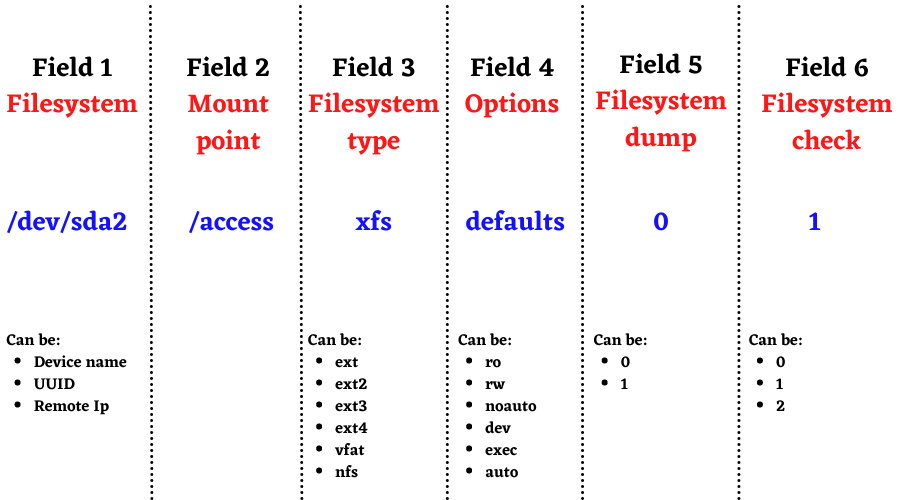
\includegraphics[scale=.5]{content/chapter8/images/fstab2.png}
		\caption{Sample /etc/fstab entries}
		\label{fstab}
	\end{figure}	
	
	\item To mount all entries from \textbf{/etc/fstab} manually, use command as shown:
	\bigskip
	\begin{tcolorbox}[breakable,notitle,boxrule=-0pt,colback=black,colframe=black]
		\color{green}
		\fontdimen2\font=1em
		\# mount -a
		\fontdimen2\font=4pt
	\end{tcolorbox}
	
	\item To know more about /etc/fstab file, check it's manual page:
	\bigskip
	\begin{tcolorbox}[breakable,notitle,boxrule=-0pt,colback=black,colframe=black]
		\color{green}
		\fontdimen2\font=1em
		\# man fstab
		\fontdimen2\font=4pt
	\end{tcolorbox}
	
\end{itemize}

\newpage
\paragraph{Understanding 6 important entries of /etc/fstab}
\bigskip
\begin{tabulary}{1.0\textwidth}{|p{5em}|p{23em}|}
	\toprule
	\textbf{Filed Name} & \textbf{Description}\\
	\midrule
	Label & Label of device to be mounted. Can be:
	\begin{itemize}
		\item Device name
		\item UUID
		\item Remote IP address
	\end{itemize}\\
	\hline
	Mount point & The directory where the filesystem will be mounted \\
	\hline
	Filesystem type & Eg: ext, ext2, ext3, xfs, vfat, swap etc. \\
	\hline
	Mount options & Permissions while mounting filesystem. Basic filesystem options are:
	\begin{itemize}
		\item \textbf{defaults}: use default options like rw, suid, dev, exec, auto, nouser, and async.
		\item \textbf{noauto}: means do not mount when "mount -a" is given (e.g., at boot time)
		\item \textbf{user}: allow a user to mount
		\item \textbf{owner}: allow device owner to mount
		\item \textbf{nofail}: do not report errors for this device if it does not exist
	\end{itemize} \\

	\bottomrule
\end{tabulary}

\newpage
\paragraph{Continue..}
\bigskip
\begin{tabulary}{1.0\textwidth}{|p{5em}|p{23em}|}
	\toprule
	\textbf{Filed Name} & \textbf{Description}\\
	\midrule
	Dump Value & Value either 0 or 1
	\begin{itemize}
		\item 0 means no backup
		\item 1 means dump utility backup of a partition
	\end{itemize}
	This is an outdated backup method and should NOT be used. \\
	\hline
	Filesystem check order & Value either 0, 1 or 2
	\begin{itemize}
		\item 0 means not to check filesystem during the Linux boot process. 
		\item The number 1 \& 2 determines the order that filesystems are checked by \textbf{fsck} during the boot process.
		\item The root directory (/) filesystem should be set to 1, and other local filesystems should be set to 2.
	\end{itemize} \\
	\bottomrule
\end{tabulary}



\end{flushleft}

\newpage

